\documentclass[a4paper, 12pt]{article}
\usepackage[utf8]{inputenc}
\usepackage[T1]{fontenc}
\usepackage{titlesec}
\usepackage{listings}
\usepackage{tikz}
\usetikzlibrary{shapes, arrows}

\tikzstyle{rect} = [rectangle, draw, minimum width=7em, minimum height=2em, rounded corners]
\tikzstyle{line} = [draw, -latex']

\lstset{basicstyle=\ttfamily, keepspaces=true}

\titleformat*{\section}{\Large\bfseries}

\title{\bf [PRI] Projekt pierwszy}
\author{Adrian Brodzik}

\begin{document}

\maketitle

\section*{Zadanie}
Napisz program, który wypisze linię znaków wejściowych zastępując każdy ciąg \textit{białych} znaków pojedynczym znakiem ukośnika, zaś ewentualne każde wystąpienie ukośnika w linii zastąpi podwójnym ukośnikiem.
\\
\\
Dla danych wejściowych:\\
\lstinline{bfvrhowev h7u893  njio nvfrowe/vtgrw         vvv}
\\
\\
Poprawnym wynikiem jest:\\
\lstinline{bfvrhowev/h7u893/njio/nvfrowe//vtgrw/vvv}

\section*{Problem}
Identyfikować ciągi białych znaków i zastępować je dokładnie jednym ukośnikiem; znajdować istniejące już wcześniej ukośniki i je duplikować.

\section*{Rozwiązanie}
Iterujemy po każdym znaku $c_{i}$ z linii znaków wejściowych. Na wyjście wypisujemy znak po znaku. Wypisujemy pojedynczy ukośnik, gdy $c_{i}$ jest znakiem białym i $c_{i-1}$ nie jest znakiem białym. Wypisujemy dwa ukosniki, gdy $c_{i}$ jest ukośnikiem. Dla znaków niebędącymi znakami białymi ani ukośnikami, wypisujemy $c_{i}$.

\section*{Biblioteka standardowa}
Użyto funkcję \texttt{printf} ze standardowej biblioteki \texttt{stdio.h} do wyświetlania komunikatów dla użytkownika oraz do wypisywania wyjścia programu.

\section*{Schemat działania}
\begin{center}
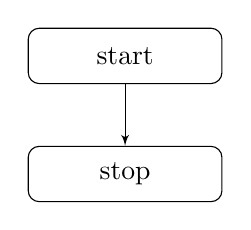
\begin{tikzpicture}[node distance = 1.5cm, auto]
\node [rect] (start) {start};
\node [rect, below of=start] (stop) {stop};
\path [line] (start) -- (stop);
\end{tikzpicture}
\end{center}

\section*{Testowanie}
Należy zwrócić uwagę na odpowiednie formatowanie wejścia programu, np. uruchamiając program
\\\\
\lstinline{> ./app some string  with   spaces    /}\\
\lstinline{Usage: app [string]}\\
\lstinline{Example: ./app "some string"}
\\\\
skutkuje błędem. Spacje w tym przypadku rozdzielają kolejne argumenty, tzn. nie wprowadzono jednej linii znaków ze spacjami, ale cztery. Poprawne uruchomienie byłoby
\\\\
\lstinline{> ./app "some string  with   spaces    /"}\\
\lstinline{some/string/with/spaces///}

\section*{Podsumowanie}
Projekt prosty służący jako wprowadzenie do języka programowania C; zapoznanie się ze składnią, typami i funkcjami sterującymi.

\end{document}
